\chapter{Background}

\section{CSR Storage Format}
CSR (Compressed Sparse Row) is the most widely used storage format for sparse matrices. As its name suggests, it compresses the amount of memory used to store a matrix without loss of information. It does so by utilizing three vectors \(A_{p}, A_{j}, A_{x}\). Figure \ref{fig:csrformat} shows an example of a matrix stored in CSR format, adapted from \cite{gupta2024gamgi}.

\begin{figure}[ht]
    \centering
    \incfig{csrformat}
    \caption{Matrix represented in the CSR format.}
    \label{fig:csrformat}
\end{figure}

The first vector, \(A_{p}\) stores the indices of the first non-zero in the vectors \(A_{p}\) and \(A_{x}\). For a given entry \(A_{p}[i]\), \(A_{p}[i]\) is the index of the first non-zero in the \(i^{\text{th}}\) row. \(A_{j}[j]\) and \(A_{x}[j]\) denotes the column index and value of the \(j^{\text{th}}\) non-zero, respectively.
\medskip

Throughout the remainder of this thesis, we operate under the assumption that all matrices are represented in CSR format, unless explicitly noted otherwise.


\subsection{Computational Intensity}

The \textit{computational intensity} of an operation describes the relation between the number of floating-point operations (FLOPS) and the number of memory accesses required. It is formally defined as:

\begin{equation}
    \text{Computational intensity} = \frac{\text{FLOPS}}{\text{Memory accesses}}
    \label{eq:computationaldensity}
\end{equation}

Operations with low computational intensity, such as SpMV, are often \textit{memory bound} rather than \textit{compute bound}. This means that increasing the computational power of a system (e.g., faster processors) does not necessarily lead to proportional speedups in SpMV performance, as memory bandwidth remains the limiting factor.

\section{Other storage formats}
There exists many other lesser used storage formats for matrices
% There are of course other ways to store a matrix, each with their own benefits and drawbacks.

\subsection{COO Format}
The Coordinate List (COO) format stores the matrix as a set of triples on the form \(i,j,x\), where \(i\) is the row index, \(j\) is the column index, and \(x\) is the value stored at \((i,j)\) in the matrix. In this format all \(0\) entries are ignored.

\begin{figure}[H]
    \centering
    \incfig{cooformat}
    \caption{Example Matrix represented in the COO format.}
    \label{fig:cooformat}
\end{figure}


\subsection{CSC Format}
The Compressed Sparse Column (CSC) format is similar to the CSR format, but instead of compressing the rows, we compress the columns. In this matrix format, we have irregular memory writes, but the reads are more regular. This can however be a problem

\begin{figure}[H]
    \centering
    \incfig{cscformat}
    \caption{Matrix represented in the CSC format.}
    \label{fig:cscformat}
\end{figure}

\subsection{ELLPack Format}
For an \(M \times  N\) matrix with a maximum of \(K\) non-zeros per row, the ELLPack format stores the non-zeros in an \(M \times  K\) matrix \texttt{data}, and an \(M \times  K\) matrix \texttt{indices}. The \texttt{data} matrix store the values of the non-zeros, and \texttt{indices} store the column index of every element. Rows that have fewer than \(K\) non-zeros are padded with zeros. Adapted from \cite{ellpackformat}.

\begin{figure}[ht]
    \centering
    \incfig{ellpackformat}
    \caption{Matrix Represented in the ELLPACK format.}
    \label{fig:ellpackformat}
\end{figure}


\section{Sequential SpMV}
A sequential implementation of SpMV on a matrix stored in the CSR format can be implemented in the following manner:
\medskip

\begin{algorithm}[htbp]
    \caption{Sequential CSR-based SpMV}
    \SetAlgoVlined
    \SetKwInOut{Input}{Input}
    \SetKwInOut{Output}{Output}
    \Input{\(A_{p},A_{j},A_{x},x\)}
    \Output{\(y\)\newline}

    \For{\(i \gets 0\) \KwTo \(n\)}{
        sum \(\gets 0\)\\
        \For{\(j \gets A_{p}[i]\) \KwTo \(A_{p}[i+1]\)}{
            sum \( = \text{sum} + A_{x}[j] \cdot x[A_{j}[j]]\)\\
        }
        \(y[i] \gets\) sum
    }
\end{algorithm}
\label{alg:sequentialspmv}
\medskip

% For SpMV on well structured matrices, i.e. those similar to the matrix shown in Figure \ref{fig:Cube_Coup_dt0}  we read 12 bytes, and perform 2 FLOPS for each non-zero in the matrix. Keen-eyed readers might notice that this does not coincide with the amount of FLOPS read per non-zero in \autoref{alg:sequentialspmv}. Here we read two doubles, and one integer, which would be equivalent to 20 bytes. The reason for the discrepancy is due to the fact that after the first time \(x\) is accessed, it is loaded into cache, and heavily reused in subsequent iterations, and can for that reason be disregarded.

% For heavily unstructured matrices, it is possible that we acutally read up to 76 bytes per 2 FLOPS. This will occur if there is no cache reuse, and a new cache line (64 bytes) is loaded for each non-zero.

For SpMV on well structured matrices such as those similar to the matrix illustrated in Figure \ref{fig:Cube_Coup_dt0}, each non-zero element typically incurs a data movement cost of approximately 12 bytes and results in 2 floating-point operations (FLOPs). This estimation may appear inconsistent with the data access pattern described in \autoref{alg:sequentialspmv}, where two double-precision values and one integer are accessed per non-zero, corresponding to a total of 20 bytes. The apparent discrepancy arises from the caching behavior of the input vector \(x\): after the initial access, elements of \(x\) are frequently reused and thus remain in cache, reducing the effective memory traffic associated with subsequent accesses.
\medskip

In contrast, for highly unstructured matrices, the absence of data locality can significantly degrade cache reuse. In the worst case scenario, each non-zero may trigger the loading of an entire 64 byte cache line, with only a small fraction of it being used. Consequently, the effective data movement can increase to as much as 76 bytes per 2 FLOPs.

\begin{figure}[H]
    \centering
    \begin{subfigure}[t]{0.45\textwidth}
        \centering
        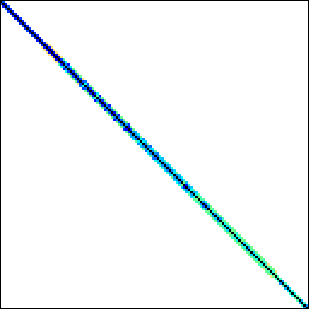
\includegraphics[width=\textwidth]{Cube_Coup_dt0}
        \caption{Cube\_Coup\_dt0}
    \end{subfigure}
    \hfill
    \begin{subfigure}[t]{0.45\textwidth}
        \centering
        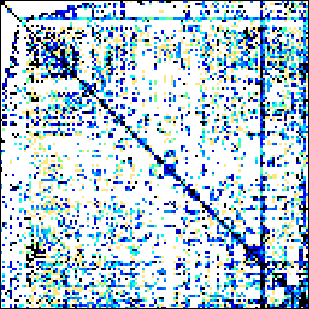
\includegraphics[width=\linewidth]{shermanACd}
        \caption{shermanACd}
    \end{subfigure}
    \caption{Well structured (a) and poorly structured (b) matrices.}
    \label{fig:Cube_Coup_dt0}
\end{figure}

\section{Shared Memory SpMV}
SpMV can be parallelized using the OpenMP directive \texttt{\#pragma omp parallel for}. By default, this tells OpenMP to use \texttt{static} scheduling when parallelizing the outer iteration loop. When static scheduling is used, the span of the iteration that each thread will execute is precomputed, and stays static, as the naming suggests. There are other scheduling options, such as \texttt{dynamic} and \texttt{guided}, which will be discussed in later sections.
\medskip

An implementation of shared memory SpMV is outlined below.
\medskip

\begin{algorithm}[H]
    \caption{Shared Memory CSR-based SpMV}
    \SetAlgoVlined
    \SetKwInOut{Input}{Input}
    \SetKwInOut{Output}{Output}
    \Input{\(A_{p},A_{j},A_{x},x\)}
    \Output{\(y\)\newline}

    \#pragma omp parallel for\\
    \For{\(i \gets 0\) \KwTo \(n\)}{
        sum \(\gets 0\)\\
        \For{\(j \gets A_{p}[i]\) \KwTo \(A_{p}[i+1]\)}{
            sum \( = \text{sum} + A_{x}[j] \cdot x[A_{j}[j]]\)\\
        }
        \(y[i] \gets\) sum
    }
    \label{alg:sharedmemoryspmv}
\end{algorithm}

\subsection{Scheduling options}
\label{sec:schedulingoptions}
As seen in \autoref{alg:sharedmemoryspmv}, the outer loop is parallelized, which translates to dividing the rows of the matrix evenly among the threads. This work fine for well structured matrices, but for matrices with dense rows, such as the matrix shown in Figure \ref{fig:staticscheduling}, we obtain large imbalances in the computational load for each thread, which impacts performance. 

\begin{figure}[H]
    \centering
    \incfig{staticscheduling}
    \caption{Row distribution among threads under static scheduling.}
    \label{fig:staticscheduling}
\end{figure}

\subsection{Dynamic Scheduling}

Dynamic scheduling in OpenMP involves precomputing the range of iterations without assigning specific iteration subsets to individual threads in advance. Under static scheduling, if thread \(A\) receives sparse rows and thread \(B\) receives dense rows, thread \(A\) will become idle prematurely while thread \(B\) remains computationally engaged. In contrast, dynamic scheduling allocates iterations at runtime to threads as they become available, thus potentially balancing the computational load more effectively, particularly when iteration workloads vary significantly.

At first glance, dynamic scheduling appears to resolve the workload imbalance inherent in static scheduling, even though it comes with more overhead. While this assumption holds true on smaller systems, such as personal laptops equipped with fewer physical cores and a single processor socket, it does not readily apply to larger, dual-socket systems utilized in this thesis. Here, the first-touch memory policy becomes particularly significant.

\subsection{First-Touch Policy}
The first-touch policy stipulates that the initial thread accessing a memory page allocates this page to its local memory domain. Consequently, if thread  first accesses a memory page, it is stored locally to thread . Subsequent accesses by thread  to this page result in non-local memory access, compelling thread  to retrieve the data from either remote or main memory. Such accesses incur performance penalties due to significantly higher latency compared to local memory access.

\subsection{Performance Implications of the First-Touch Policy}

Table \ref{tab:latencynumbers} illustrates that accesses to main memory exhibit substantially higher latency compared to local cache (e.g., L1 cache) accesses. In dual-socket configurations, accessing memory residing on the remote socket involves inter-socket communication through an interlink, further exacerbating latency. Consequently, dynamic (or guided) scheduling alone does not mitigate the performance degradation arising from poorly structured matrices, as it inadvertently exacerbates memory locality issues inherent to the first-touch policy on NUMA architectures.








% This algorithm can be parallelized using shared memory parallelization using OpenMPs \texttt{\#pragma omp parallel for} directive in the following manner:
% \medskip

% \begin{algorithm}[H]
%     \caption{Sequential CSR-based SpMV}
%     \SetAlgoVlined
%     \SetKwInOut{Input}{Input}
%     \SetKwInOut{Output}{Output}
%     \Input{\(A_{p},A_{j},A_{x},x\)}
%     \Output{\(y\)\newline}

%     \textbf{\#pragma omp parallel for}\\
%     \For{\(i \gets 0\) \KwTo \(n\)}{
%         \(y[i] \gets 0\)\\
%         \For{\(j \gets A_{p}[i]\) \KwTo \(A_{p}[i+1]\)}{
%             \(y[i] \gets y[i] + A_{x}[j] \cdot x[A_{j}[j]]\)\\
%         }
%     }
% \end{algorithm}

% \section{Computational Intensity}

\section{Distributed Memory SpMV}
In distributed memory systems, the computational workload is distributed across multiple nodes, each typically comprising a dual-socket architecture with local memory. Unlike shared memory systems, data access across nodes is non-trivial and requires explicit communication, most commonly implemented using the Message Passing Interface (MPI).

For distributed sparse matrix-vector multiplication (SpMV), the computation proceeds similarly to the shared memory case (\autoref{alg:sharedmemoryspmv}). The sparse matrix is divided across nodes, and each node computes its local segment of the output vector \(y\). At the end of each iteration, partial results are assembled to produce the global vector, necessitating inter-node communication.

\medskip

While the thread scheduling and memory locality issues discussed in \ref{sec:schedulingoptions} remain relevant, distributed memory systems introduce the additional challenge of communication overhead. As shown in Table \ref{tab:latencynumbers}, inter-node communication is significantly more expensive than memory accesses. Consequently, minimizing the total communication volume per SpMV iteration is critical for performance.


\subsection{Load Balancing and Graph Partitioning}
Even with a well-balanced distribution, excessive communication between nodes can become a performance bottleneck if data dependencies span many partitions. An effective partitioning strategy must therefore strike a careful balance between distributing the computational load evenly and reducing the amount of communication required between ranks. This trade-off is naturally captured by the graph partitioning problem.
\medskip

The graph partitioning problem involes dividing an undirected graph \(G(V,E)\), where \(V\) is the set of vertices and \(E\) is the set of edges into \(K\) disjoint subsets (or partitions) such that each subset contains a comparable amount of vertices, and the number of edges connecting different subsets is minimized. Each vertex \(v_{i} \in V\) may be assigned a weight \(w_{i}\), and each edge \(e_{ij} \in E\) may carry a cost \(c_{ij}\). The sum of weights \(W_{k}\) of each partition \(P_{k}\) must not exceed a specified imbalance threshold \(\epsilon\) relative to the average weight of each partition. An edge can be classified as either an internal edge (those that connect nodes in the same partition), or an external edge (those that connect vertices in different partitions), and the cutsize is defined as the sum of the costs of all external edges. The goal is to minize the cutsize, while preserving the balance between the size of each partition. This problem is known to be NP-Hard, even for obtaining bipartitions on unweighted graphs (adapted from \cite{hypergraphpartitioning}).
\medskip

Algorithms that aim to solve the graph partitioning problem rely on heuristics that provide good approximations in practice. Optimizing for one objective at the expense of the other is trivial but undesirable: assigning all vertices to a single partition minimizes communication to zero but results in extreme load imbalance, whereas naïvely assigning vertices to maintain balance without regard to connectivity may lead to high communication costs.

\subsection{METIS}
The graph partitioner used for the experiments in this thesis is called METIS. METIS is a software package for partitioning large irregular graphs, and has other uses such as partitioning meshes and computing fill-reducing orderings of sparse matrices. METIS provides algorithms that are based on multilevel graph partitoning. These algorithms partition the graph through a coarsening and refinement phase. In the coarsening phase, the size of the graph is reduced by way of collapsing the vertices and edges, and then partition the smaller graph. In the refinement phase, the graph is gradually expanded to its original size, and the portion of the graph that is close to the boundary is the primary focus, ensuring the quality of the partition is kept (adapted from \cite{karypis1997metis}).
\medskip

The way METIS partitions graph does not necessarily optimize for minimizing the communication volume, but rather obtaining partitions that are roughly equal in size. It is possible that there are partitions that have a larger imbalance between the size of partitions, but much smaller communication volumes. In order to obtain partitions that optimize for minimizing communication, it is necessary to look to hypergraph partitioners.

\begin{figure}[H]
    \centering
    \incfig{coarseninggraph}
    \caption{Illustration of multilevel graph partitioning.}
    \label{fig:coarseninggraph}
\end{figure}

\subsubsection{Hypergraph Partitioning}




% Algorithm~\ref{alg:partitioning} outlines the procedure used to partition a sparse matrix using METIS and reorder its rows and columns to reflect the resulting partition layout. This reordering ensures that each partition corresponds to a contiguous block of rows, improving data locality and facilitating parallel distribution.
\begin{algorithm}[H]
    \caption{Partitioning and reordering a matrix.}
    \label{alg:partitioning}
    \SetAlgoVlined
    \SetKwInOut{Input}{Input}
    \SetKwInOut{Output}{Output}
    \Input{\(g\), \(n_{p}\), \(p\) }
    \Output{Partitioned and reordered \(g\)\newline}

    \If{\(n_{p} = 1\)}{
        p[0] \(\gets\) 0 \\
        p[1] \(\gets\) \(g.n_{r}\)\\
        \KwRet \(g\) \\
    }

    partitionVector \(\gets\) METIS\_PartGraphKway(\texttt{arguments specifying constraints for partition})\\

    newId \(\gets [0] \cdot g.n_{r}\)\\
    oldId \(\gets [0] \cdot g.n_{r}\)\\
    id \(\gets\) 0 \\
    p[0] \(\gets\) 0 \\

    \For{\(r \in \left\{ 0, \dots r \right\}\)}{
        \For{\(i \in \left\{ 0, \dots , g.n_{r} \right\}\)}{
            \If {partitionVector[\(i\)] = \(r\)}{
                oldId[\(id\)] \(\gets i\)\\
                newId[\(i\)] \(\gets\) id\\
                id \(\gets\) id + 1\\
            }
        }
        partitionVector[\(r + 1\)] \(\gets\) id\\
    }

    newRowPtr \(\gets [0] \cdot g.n_{r} + 1\)\\
    newColIdx \(\gets [0] \cdot g.n_{c}\)\\
    newValues \(\gets [0] \cdot g.n_{c}\)\\


    \For{\(i \in \{0, \dots , g.n_{r}-1\}\)}{
        d \(\gets\) g.rowPtr[oldId[i]+1] - g.rowPtr[oldId[i]]\\
        newRowPtr[i + 1] \(\gets\) newRowPtr[i] + d\\

        \For{\(j \in \{0, \dots , d - 1\}\)}{
            newColIdx[newRowPtr[i] + j] \(\gets\) g.colIdx[g.rowPtr[oldId[i]] + j]\\
            newValues[newRowPtr[i] + j] \(\gets\) g.values[g.rowPtr[oldId[i]] + j]\\
        }

        \For{\(j \in \{newRowPtr[i], \dots , newRowPtr[i+1]-1\}\)}{
            newColIdx[j] \(\gets\) newId[newColIdx[j]]\\
        }
    }

    g.rowPtr \(\gets\) newRowPtr\\
    g.colIdx \(\gets\) newColIdx\\
    g.values \(\gets\) newValues\\

    \KwRet g\\
\end{algorithm}


% In order to reduce the total communication volume, tools such as graph partiotioners or hypergraph partitioners are often used. These tools
% A big factor in reducing the communication volume 

% In a distributed memory system, it is important to partition the matrix so that the computational workload is evenly divided among the processes. This is typically achieved through the use of graph partitioning tools. A widely used tool for this purpose is METIS, which provides the function \texttt{METIS\_PartGraphKway}. Given a parameter \(nprocs\), representing the number of procsses the program will run on, \texttt{METIS\_PartGraphKway} attempts to partition the graph into \(nprocs\) equally sized parts. Since finding an optimal partition is an NP-hard problem, METIS does not guarantee an optimal solution, but it produces high-quality approximations that are sufficient for practical use.

% \subsection{Separator}
% When a graph is partitioned into different parts, there will inevitably be some edges which strides across different partitions. The endpoints of these edges are called separators, and will become important when it comes to reducing the communication load of the SpMV computation.
